% So I have up to 11 texts I need to show here
% lut64
% pext64
% shuffle64
% shuffle128
% shuffle256
% shuffle512
% pc
% pc-ss
% ps
% kaneta-pext
% kaneta-pshufb

\documentclass[a4]{article}

\usepackage[utf8]{inputenc}
\usepackage[english]{babel}

\usepackage{amsmath,amsfonts,amssymb}
\usepackage{fullpage}
\usepackage{verbatim}

\usepackage{tikz,pgfplots}
\usetikzlibrary{patterns, patterns.meta}
\usepgfplotslibrary{groupplots}



\pgfplotsset{
    major grid style = { thin, dotted, color = black!50 },
    minor grid style = { thin, dotted, color = black!50 },
    grid,
    xtick distance = 1,
    ymin = 0,
    legend cell align = left,
    legend pos = north west,
	  /pgfplots/ybar legend/.style = {
		  /pgfplots/legend image code/.code={%
			  \draw[##1,/tikz/.cd,yshift=-0.35em]
      (0cm,0cm) rectangle (0.7em,0.8em);},
	  },  
}


\begin{document}

\title{WT Benchmark}
\author{Jan-Philipp Tarnowski}
\maketitle

\clearpage

% Okay, this will be fun

% IMPORT-DATA stats ../final/results-pcc-huff-sans-sources-pitches.out
% IMPORT-DATA stats_b ../final/results-pcc-huff-sources.out
% IMPORT-DATA stats_c ../final/results-pcc-huff-pitches-no-wm-pc.out
% IMPORT-DATA stats_d ../final/results-lightweight-huff-chr22-gcc-30-jdk13c-rfc-w3c-rctail96.out
% IMPORT-DATA stats_e ../final/results-lightweight-huff-etexthowto-linux-sans-wx-pc.out
% IMPORT-DATA stats_f ../final/results-lightweight-huff-sprot.out


% SQL INSERT INTO stats SELECT * FROM stats_b
% SQL INSERT INTO stats SELECT * FROM stats_c
% SQL INSERT INTO stats SELECT * FROM stats_d
% SQL INSERT INTO stats SELECT * FROM stats_e
% SQL INSERT INTO stats SELECT * FROM stats_f

% Post large texts 

% IMPORT-DATA stats_x_a ../final/results-huff-pcc-2.out
% IMPORT-DATA stats_x_b ../final/results-huff-lightweight-2.out
% IMPORT-DATA stats_x_c ../final/results-huff-large-mawt.out
% IMPORT-DATA stats_x_d ../final/results-huff-wc-large-sans-pc-matrix.out
% IMPORT-DATA stats_x_e ../final/results-huff-pc-wm-large.out

% SQL DELETE FROM stats WHERE type LIKE 'lwt%'
% SQL DELETE FROM stats WHERE type LIKE 'wm%'

% SQL INSERT INTO stats SELECT * FROM stats_x_a
% SQL INSERT INTO stats SELECT * FROM stats_x_b
% SQL INSERT INTO stats SELECT * FROM stats_x_c
% SQL INSERT INTO stats SELECT * FROM stats_x_d
% SQL INSERT INTO stats SELECT * FROM stats_x_e

% SQL UPDATE stats SET type = 'lwt-huff-pext-16-4', ds_order = 0 WHERE type LIKE 'lwt_huffman_pext_16_4'
%~ SQL UPDATE stats SET type = 'lwt-huff-shuffle-8-8', ds_order = 1 WHERE type LIKE 'lwt_huffman_shuffle_8_8'
%~ SQL UPDATE stats SET type = 'lwt-huff-shuffle-16-8', ds_order = 2 WHERE type LIKE 'lwt_huffman_shuffle_16_8'
%~ SQL UPDATE stats SET type = 'lwt-huff-shuffle-32-8', ds_order = 3 WHERE type LIKE 'lwt_huffman_shuffle_32_8'
% SQL UPDATE stats SET type = 'lwt-huff-shuffle-64-8', ds_order = 4 WHERE type LIKE 'lwt_huffman_shuffle_64_8'
% SQL UPDATE stats SET type = 'lwt-pwm-huff-pc', ds_order = 5 WHERE type LIKE 'pwm_%wx_huff_pc________tree_huffman'
% SQL UPDATE stats SET type = 'lwt-pwm-huff-pc-ss', ds_order = 6 WHERE type LIKE 'pwm_%wx_huff_pc_ss________tree_huffman'
% SQL UPDATE stats SET type = 'lwt-pwm-huff-ps', ds_order = 7 WHERE type LIKE 'pwm_%wx_huff_ps________tree_huffman'

% SQL UPDATE stats SET type = 'wm-huff-pext-16-4', ds_order = 8 WHERE type LIKE 'wm_huffman_pext_16_4'
%~ SQL UPDATE stats SET type = 'wm-huff-shuffle-8-8', ds_order = 9 WHERE type LIKE 'wm_huffman_shuffle_8_8'
%~ SQL UPDATE stats SET type = 'wm-huff-shuffle-16-8', ds_order = 10 WHERE type LIKE 'wm_huffman_shuffle_16_8'
%~ SQL UPDATE stats SET type = 'wm-huff-shuffle-32-8', ds_order = 11 WHERE type LIKE 'wm_huffman_shuffle_32_8'
% SQL UPDATE stats SET type = 'wm-huff-shuffle-64-8', ds_order = 12 WHERE type LIKE 'wm_huffman_shuffle_64_8'
% SQL UPDATE stats SET type = 'wm-pwm-huff-pc', ds_order = 13 WHERE type LIKE 'pwm_%wx_huff_pc________matrix_huffman'
% SQL UPDATE stats SET type = 'wm-pwm-huff-pc-ss', ds_order = 14 WHERE type LIKE 'pwm_%wx_huff_pc_ss________matrix_huffman'
% SQL UPDATE stats SET type = 'wm-pwm-huff-ps', ds_order = 15 WHERE type LIKE 'pwm_%wx_huff_ps________matrix_huffman'

% SQL DELETE FROM stats WHERE type LIKE '%\_%' ESCAPE '\'

% IMPORT-DATA text_info ../final/results-stats.log

% SQL CREATE TABLE stats_joined AS SELECT * FROM stats JOIN text_info ON stats.file = text_info.file
% SQL DROP TABLE stats
% SQL ALTER TABLE stats_joined RENAME TO stats

% SQL UPDATE stats SET file = 'dblp.xml' WHERE file LIKE '%/dblp.xml'
% SQL UPDATE stats SET file = 'dna' WHERE file LIKE '%/dna'
% SQL UPDATE stats SET file = 'english' WHERE file LIKE '%/english'
% SQL UPDATE stats SET file = 'pitches' WHERE file LIKE '%/pitches'
% SQL UPDATE stats SET file = 'proteins' WHERE file LIKE '%/proteins'
% SQL UPDATE stats SET file = 'sources' WHERE file LIKE '%/sources'

% SQL UPDATE stats SET file = 'chr22.dna' WHERE file LIKE '%/chr22.dna'
% SQL UPDATE stats SET file = 'etext99' WHERE file LIKE '%/etext99'
% SQL UPDATE stats SET file = 'gcc-3.0.tar' WHERE file LIKE '%/gcc-3.0.tar'
% SQL UPDATE stats SET file = 'howto' WHERE file LIKE '%/howto'
% SQL UPDATE stats SET file = 'jdk13c' WHERE file LIKE '%/jdk13c'
% SQL UPDATE stats SET file = 'linux-2.4.5.tar' WHERE file LIKE '%/linux-2.4.5.tar'
% SQL UPDATE stats SET file = 'rctail96' WHERE file LIKE '%/rctail96'
% SQL UPDATE stats SET file = 'rfc' WHERE file LIKE '%/rfc'
% SQL UPDATE stats SET file = 'sprot34.dat' WHERE file LIKE '%/sprot34.dat'
% SQL UPDATE stats SET file = 'w3c2' WHERE file LIKE '%/w3c2'

% SQL UPDATE stats SET file = 'cc.16gib' WHERE file LIKE '%/cc.txt'
% SQL UPDATE stats SET file = 'dna.16gib' WHERE file LIKE '%/dna.txt'
% SQL UPDATE stats SET file = 'wiki.16gib' WHERE file LIKE '%/wiki.txt'
% SQL UPDATE stats SET file = 'ru.8gib' WHERE file LIKE '%/ru.wo_punct.wb'

% SQL DELETE FROM stats WHERE file NOT like '%gib'

\pgfplotsset{
  /pgfplots/bar cycle list/.style = {
    /pgfplots/cycle list = {
      { fill = green!65, mark = none },        % PEXT
      { fill = blue!55, mark = none },         % PSHUFB 8-8
      { fill = orange!65, mark = none },       % PSHUFB 16-8
      { fill = violet!60, mark = none },       % PSHUFB 32-8
      { fill = yellow!80, mark = none },       % PSHUFB 64-8
      { fill = blue!50!green!75, mark = none },% PWM PC
      { fill = red!75!blue!50, mark = none },  % PWM PC SS
      { fill = brown!50, mark = none }         % PWM PS
    }
  }
}


\centering
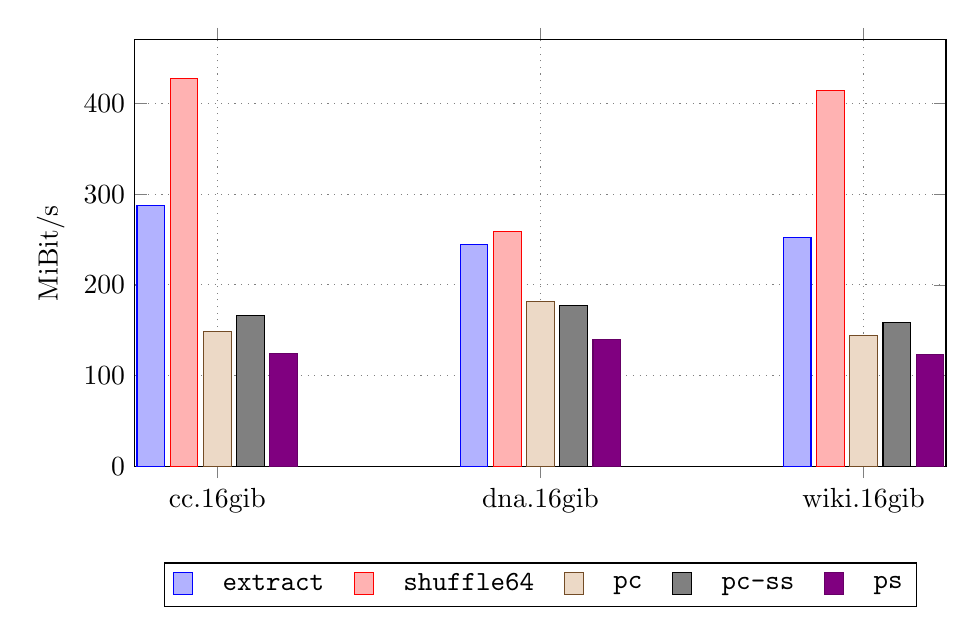
\begin{tikzpicture}
    \begin{axis} [
        width = 0.98\textwidth,
        height = 7.0cm,
        ybar,
        enlarge x limits = 0.1275,
        ylabel = MiBit/s,
        legend style = { 
            at = {(0.5, -0.225)},
            anchor = north,
            legend columns = 5,
            column sep = 2ex
        },
        ytick distance = 100,
        symbolic x coords = {
            %dblp.xml,
            %dna,
            %english,
            %pitches,
            %proteins,
            %sources,
            %chr22.dna,
            %etext99,
            %gcc-3.0.tar,
            %howto,
            %jdk13c,
            %linux-2.4.5.tar,
            %rctail96,
            %rfc,
            %sprot34.dat,
            %w3c2,
            cc.16gib,
            dna.16gib,
            wiki.16gib
            %ru.8gib
        }
    ]
    
    
  
  %% MULTIPLOT(type) SELECT file AS x, MEDIAN((huff_bit_size / CAST(time_in_s AS FLOAT)) / (1024 * 1024)) AS y,MULTIPLOT
  %% FROM stats WHERE (type LIKE 'lwt%') GROUP BY MULTIPLOT,x ORDER BY ds_order,MULTIPLOT,x
  \addplot coordinates { (cc.16gib,287.724) (dna.16gib,244.315) (wiki.16gib,251.961) };
  \addlegendentry{type=lwt-huff-pext-16-4};
  \addplot coordinates { (cc.16gib,427.436) (dna.16gib,258.727) (wiki.16gib,414.723) };
  \addlegendentry{type=lwt-huff-shuffle-64-8};
  \addplot coordinates { (cc.16gib,148.24) (dna.16gib,182.211) (wiki.16gib,144.614) };
  \addlegendentry{type=lwt-pwm-huff-pc};
  \addplot coordinates { (cc.16gib,166.164) (dna.16gib,177.096) (wiki.16gib,158.651) };
  \addlegendentry{type=lwt-pwm-huff-pc-ss};
  \addplot coordinates { (cc.16gib,124.803) (dna.16gib,139.916) (wiki.16gib,122.848) };
  \addlegendentry{type=lwt-pwm-huff-ps};



        \legend {
            \texttt{extract},
            %\texttt{shuffle8},
            %\texttt{shuffle16},
            %\texttt{shuffle32},
            \texttt{shuffle64},
            \texttt{pc},
            \texttt{pc-ss},
            \texttt{ps}
        }
      
    \end{axis}
\end{tikzpicture}

\centering
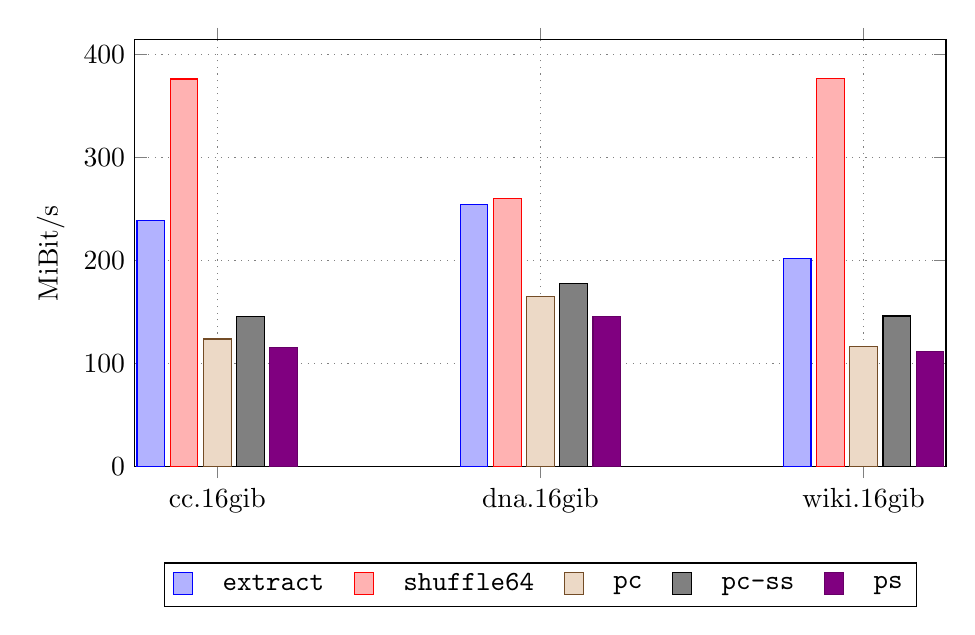
\begin{tikzpicture}
    \begin{axis} [
        width = 0.98\textwidth,
        height = 7.0cm,
        ybar,
        enlarge x limits = 0.1275,
        ylabel = MiBit/s,
        legend style = { 
            at = {(0.5, -0.225)},
            anchor = north,
            legend columns = 5,
            column sep = 2ex
        },
        ytick distance = 100,
        symbolic x coords = {
            %dblp.xml,
            %dna,
            %english,
            %pitches,
            %proteins,
            %sources,
            %chr22.dna,
            %etext99,
            %gcc-3.0.tar,
            %howto,
            %jdk13c,
            %linux-2.4.5.tar,
            %rctail96,
            %rfc,
            %sprot34.dat,
            %w3c2,
            cc.16gib,
            dna.16gib,
            wiki.16gib
            %ru.8gib
        }
    ]
    
    
  
  %% MULTIPLOT(type) SELECT file AS x, MEDIAN((huff_bit_size / CAST(time_in_s AS FLOAT)) / (1024 * 1024)) AS y,MULTIPLOT
  %% FROM stats WHERE (type LIKE 'wm%') GROUP BY MULTIPLOT,x ORDER BY ds_order,MULTIPLOT,x
  \addplot coordinates { (cc.16gib,238.825) (dna.16gib,254.081) (wiki.16gib,201.598) };
  \addlegendentry{type=wm-huff-pext-16-4};
  \addplot coordinates { (cc.16gib,376.079) (dna.16gib,260.218) (wiki.16gib,376.514) };
  \addlegendentry{type=wm-huff-shuffle-64-8};
  \addplot coordinates { (cc.16gib,123.683) (dna.16gib,164.914) (wiki.16gib,116.729) };
  \addlegendentry{type=wm-pwm-huff-pc};
  \addplot coordinates { (cc.16gib,145.789) (dna.16gib,177.848) (wiki.16gib,146.057) };
  \addlegendentry{type=wm-pwm-huff-pc-ss};
  \addplot coordinates { (cc.16gib,115.757) (dna.16gib,145.117) (wiki.16gib,111.705) };
  \addlegendentry{type=wm-pwm-huff-ps};



        \legend {
            \texttt{extract},
            %\texttt{shuffle8},
            %\texttt{shuffle16},
            %\texttt{shuffle32},
            \texttt{shuffle64},
            \texttt{pc},
            \texttt{pc-ss},
            \texttt{ps}
        }
      
    \end{axis}
\end{tikzpicture}

\end{document}


